\section{Seismic Networks}


%----------------------------------------------------------------%
\begin{frame}{Graph example of a Seismic Network}

\begin{figure}[h]
\begin{subfigure}[b]{0.4\linewidth}
\centering
\resizebox{0.95\textwidth}{!}{%
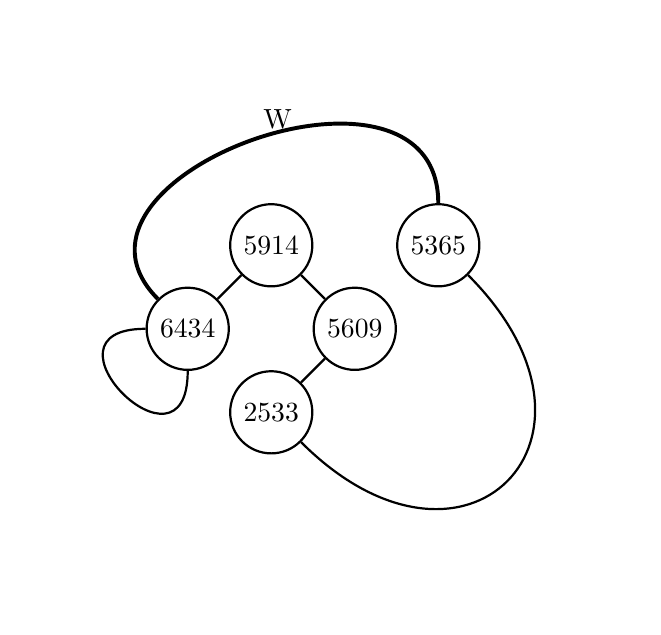
\begin{tikzpicture}[node distance={15mm}, thick, main/.style = {draw, circle}] 
\node[main] (1) {$6434$}; 
\node[main] (2) [above right of=1] {$5914$}; 
\node[main] (3) [below right of=1] {$2533$}; 
\node[main] (4) [above right of=3] {$5609$}; 
\node[main] (5) [above right of=4] {$5365$}; 

\draw(1) -- (2); 
%\draw(1) -- (3); 
\draw [line width=0.05cm] (1) to [out=135,in=90,looseness=1.5] node[midway, above right] {W}  (5); 
\draw (1) to [out=180,in=270,looseness=5] (1); 
\draw (2) -- (4); 
\draw (3) -- (4); 
%\draw (5) -- (4); 
\draw (5) to [out=315, in=315, looseness=2.5]  (3); 
\end{tikzpicture}}
\end{subfigure}
\begin{subfigure}[b]{0.4\linewidth}
  \includegraphics[width=\textwidth]{quakesTable2}
  \label{fig:qTab2}
\end{subfigure}%

\caption{Seismic Network (Graph representation) example: Nodes are identified as $cubeIndex$, used to acces any information about events in that respective cube from our Earthquakes Table. Edge weight can be represented on the edge as $W$, where each additional link between two nodes increases this value by 1.}
\end{figure}

\end{frame}


%----------------------------------------------------------------%
\begin{frame}{Connectivity of a Network}
The fundamental measure to describe our seismic network is the connectivity distribution $P(k)$. This distribution comes naturally by realising the histogram of the nodes degree and then the regression of the distribution and show that it follows a power law:

\begin{equation}
P(k) \sim k^{-\gamma}
\end{equation}

The connectivity computations are made for various seismic networks (Vrancea(Romania), California(USA), Italy and Japan), with different magnitude restrictions, for 2 cube sizes: $5\times5\times5$ km and $10\times10\times10$ km, with and without edge weights.
\end{frame}


% ---------------------------- VRANCEA CONNECTIVITY ----------------------------%
%----------------------------------------------------------------%
\begin{frame}{Vrancea Connectivity}
\begin{figure}[!h]
\begin{subfigure}{.5\textwidth}
  \includegraphics[width=\textwidth]{connectivityVrancea_1magnitude10}
  \caption{$1 \leq magnitude$}
  \label{fig:conVr1mag10}
\end{subfigure}%
\hfill
\begin{subfigure}{.5\textwidth}
  \includegraphics[width=\textwidth]{connectivityVrancea_2magnitude10}
  \caption{$2 \leq magnitude$}
  \label{fig:conVr2mag10}
\end{subfigure}%

\vskip\baselineskip

\begin{subfigure}{.5\textwidth}
  \includegraphics[width=\textwidth]{connectivityVrancea_2magnitude4}
  \caption{$2\leq magnitude \leq 4$}
  \label{fig:conVr2mag14}
\end{subfigure}%
\hfill
\begin{subfigure}{.5\textwidth}
  \includegraphics[width=\textwidth]{connectivityVrancea_3magnitude7}
  \caption{$3 \leq magnitude \leq 7$}
  \label{fig:conVr3mag7}
\end{subfigure}%

\caption{Connectivity distribution $P(k)$ for Vrancea in log-log and interpolation of the results, for a number of magnitude ranges. The exponent of the power law, $\gamma$ ranges from $\sim 1.08$ to $1.756$.}
\label{fig:connectivityVr}
\end{figure}
\end{frame}


%----------------------------------------------------------------%
\begin{frame}{Vrancea Weighted Connectivity}
\begin{figure}[!h]
\begin{subfigure}{.5\textwidth}
  \includegraphics[width=\columnwidth]{connectivityVranceaWeighted_1magnitude10}
  \caption{$1 \leq magnitude$}
  \label{fig:conWeiVr1mag10}
\end{subfigure}%
\hfill
\begin{subfigure}{.5\textwidth}
  \includegraphics[width=\columnwidth]{connectivityVranceaWeighted_2magnitude10}
  \caption{$2 \leq magnitude$}
  \label{fig:conWeiVr2mag10}
\end{subfigure}%

\vskip\baselineskip

\begin{subfigure}{.5\textwidth}
  \includegraphics[width=\columnwidth]{connectivityVranceaWeighted_2magnitude4}
  \caption{$2\leq magnitude \leq 4$}
  \label{fig:conWeiVr2mag4}
\end{subfigure}%
\hfill
\begin{subfigure}{.5\textwidth}
  \includegraphics[width=\columnwidth]{connectivityVranceaWeighted_3magnitude7}
  \caption{$3 \leq magnitude \leq 7$}
  \label{fig:conWeiVr3mag7}
\end{subfigure}%

\caption{Weighted connectivity distribution $P(k)$ for Vrancea in log-log and interpolation of the results, for a number of magnitude ranges. The exponent of the power law, $\gamma$ ranges from $\sim 1.95$ to $3.26$.}
\label{fig:connectivityVrWeighted}
\end{figure}
\end{frame}


% ---------------------------- California CONNECTIVITY ----------------------------%
%----------------------------------------------------------------%
\begin{frame}{California Connectivity}
\begin{figure}[!h]
\begin{subfigure}{.5\textwidth}
  \includegraphics[width=\columnwidth]{connectivityCalifornia_1magnitude10}
  \caption{$1 \leq magnitude$}
  \label{fig:conCa1mag10}
\end{subfigure}%
\hfill
\begin{subfigure}{.5\textwidth}
  \includegraphics[width=\columnwidth]{connectivityCalifornia_2magnitude10}
  \caption{$2\leq magnitude$}
  \label{fig:conCa2mag10}
\end{subfigure}%

\vskip\baselineskip

\begin{subfigure}{.5\textwidth}
  \includegraphics[width=\columnwidth]{connectivityCalifornia_1magnitude3}
  \caption{$1 \leq magnitude \leq 3$}
  \label{fig:conCa1mag3}
\end{subfigure}%
\hfill
\begin{subfigure}{.5\textwidth}
  \centering
  \includegraphics[width=\columnwidth]{connectivityCalifornia_2magnitude4}
  \caption{$2 \leq magnitude \leq 4$}
  \label{fig:conCa2mag4}
\end{subfigure}%

\caption{Connectivity distribution $P(k)$ for California in log-log and interpolation of the results, for a number of magnitude ranges. The exponent of the power law, $\gamma$ ranges from $\sim 1.45$ to $2.16$.}
\label{fig:connectivityCa}
\end{figure}
\end{frame}


%----------------------------------------------------------------%
\begin{frame}{California - Connectivity Weighted}
\begin{figure}[!h]
\begin{subfigure}{.5\textwidth}
  \includegraphics[width=\columnwidth]{connectivityCaliforniaWeighted_1magnitude10}
  \caption{$1 \leq magnitude$}
  \label{fig:conWeiCa1mag10}
\end{subfigure}%
\hfill
\begin{subfigure}{.5\textwidth}
  \includegraphics[width=\columnwidth]{connectivityCaliforniaWeighted_2magnitude10}
  \caption{$2\leq magnitude$}
  \label{fig:conWeiCa2mag10}
\end{subfigure}%

\vskip\baselineskip

\begin{subfigure}{.5\textwidth}
  \includegraphics[width=\columnwidth]{connectivityCaliforniaWeighted_1magnitude3}
  \caption{$1 \leq magnitude \leq 3$}
  \label{fig:conWeiCa1mag3}
\end{subfigure}%
\hfill
\begin{subfigure}{.5\textwidth}
  \includegraphics[width=\columnwidth]{connectivityCaliforniaWeighted_2magnitude4}
  \caption{$2 \leq magnitude \leq 4$}
  \label{fig:conWeiCa2mag4}
\end{subfigure}%

\caption{Weighted connectivity distribution $P(k)$ for California in log-log and interpolation of the results, for a number of magnitude ranges. The exponent of the power law, $\gamma$ ranges from $\sim 2.06$ to $2.71$.}
\label{fig:connectivityCaWeighted}
\end{figure}
\end{frame}


% ---------------------------- Italy CONNECTIVITY ----------------------------%
%----------------------------------------------------------------%
\begin{frame}{Italy - Connectivity}
\begin{figure}[!h]
\begin{subfigure}{.5\textwidth}
  \includegraphics[width=\columnwidth]{connectivityItaly_1magnitude10}
  \caption{$1 \leq magnitude$}
  \label{fig:conIt1mag10}
\end{subfigure}%
\hfill
\begin{subfigure}{.5\textwidth}
  \includegraphics[width=\columnwidth]{connectivityItaly_2magnitude10}
  \caption{$2\leq magnitude$}
  \label{fig:conIt2mag10}
\end{subfigure}%

\vskip\baselineskip

\begin{subfigure}{.5\textwidth}
  \includegraphics[width=\columnwidth]{connectivityItaly_1magnitude3}
  \caption{$1 \leq magnitude \leq 3$}
  \label{fig:conIt1mag3}
\end{subfigure}%
\hfill
\begin{subfigure}{.5\textwidth}
  \includegraphics[width=\columnwidth]{connectivityItaly_2magnitude4}
  \caption{$2 \leq magnitude \leq 4$}
  \label{fig:conIt2mag4}
\end{subfigure}%

\caption{Connectivity distribution $P(k)$ for Italy in log-log and interpolation of the results, for a number of magnitude ranges. The exponent of the power law, $\gamma$ ranges from $\sim 1.44$ to $2.3$.}
\label{fig:connectivityIt}
\end{figure}
\end{frame}


%----------------------------------------------------------------%
\begin{frame}{Italy - Connectivity Weighted}
\begin{figure}[!h]
\begin{subfigure}{.5\textwidth}
  \includegraphics[width=\columnwidth]{connectivityItalyWeighted_1magnitude10}
  \caption{$1 \leq magnitude$}
  \label{fig:conWeiIt1mag10}
\end{subfigure}%
\hfill
\begin{subfigure}{.5\textwidth}
  \centering
  \includegraphics[width=\columnwidth]{connectivityItalyWeighted_2magnitude10}
  \caption{$1 \leq magnitude$}
  \label{fig:conWeiIt2mag10}
\end{subfigure}%

\vskip\baselineskip

\begin{subfigure}{.5\textwidth}
  \includegraphics[width=\columnwidth]{connectivityItalyWeighted_1magnitude3}
  \caption{$1 \leq magnitude \leq 3$}
  \label{fig:conWeiIt1mag3}
\end{subfigure}%
\hfill
\begin{subfigure}{.5\textwidth}
  \includegraphics[width=\columnwidth]{connectivityItalyWeighted_2magnitude4}
  \caption{$2 \leq magnitude \leq 4$}
  \label{fig:conWeiIt2mag4}
\end{subfigure}%

\caption{Weighted connectivity distribution $P(k)$ for Italy in log-log and interpolation of the results, for a number of magnitude ranges. The exponent of the power law, $\gamma$ ranges from $\sim 2.8$ to $3.72$.}
\label{fig:connectivityItWeighted}
\end{figure}
\end{frame}


% ---------------------------- Japan CONNECTIVITY ----------------------------%
%----------------------------------------------------------------%
\begin{frame}{Japan - Connectivity}
\begin{figure}[!h]
\begin{subfigure}{.5\textwidth}
  \includegraphics[width=\columnwidth]{connectivityJapan_1magnitude10}
  \caption{$1 \leq magnitude$}
  \label{fig:conJa1mag10}
\end{subfigure}%
\hfill
\begin{subfigure}{.5\textwidth}
  \includegraphics[width=\columnwidth]{connectivityJapan_2magnitude10}
  \caption{$2\leq magnitude$}
  \label{fig:conJa2mag10}
\end{subfigure}%

\vskip\baselineskip

\begin{subfigure}{.5\textwidth}
  \includegraphics[width=\columnwidth]{connectivityJapan_1magnitude3}
  \caption{$1 \leq magnitude \leq 3$}
  \label{fig:conJa1mag3}
\end{subfigure}%
\hfill
\begin{subfigure}{.5\textwidth}
  \includegraphics[width=\columnwidth]{connectivityJapan_2magnitude4}
  \caption{$2 \leq magnitude \leq 4$}
  \label{fig:conJa2mag4}
\end{subfigure}%

\caption{Connectivity distribution $P(k)$ for Japan in log-log and interpolation of the results, for a number of magnitude ranges. The exponent of the power law, $\gamma$ ranges from $\sim 1.87$ to $2.5$.}
\label{fig:connectivityJa}
\end{figure}
\end{frame}


%----------------------------------------------------------------%
\begin{frame}{Japan - Connectivity Weighted}
\begin{figure}[!h]
\begin{subfigure}{.5\textwidth}
  \includegraphics[width=\columnwidth]{connectivityJapanWeighted_1magnitude10}
  \caption{$1 \leq magnitude$}
  \label{fig:conWeiJa1mag10}
\end{subfigure}%
\hfill
\begin{subfigure}{.5\textwidth}
  \centering
  \includegraphics[width=\columnwidth]{connectivityJapanWeighted_2magnitude10}
  \caption{$2\leq magnitude$}
  \label{fig:conWeiJa2mag10}
\end{subfigure}%

\vskip\baselineskip

\begin{subfigure}{.5\textwidth}
  \includegraphics[width=\columnwidth]{connectivityJapanWeighted_1magnitude3}
  \caption{$1\leq magnitude \leq 3$}
  \label{fig:conWeiJa1mag3}
\end{subfigure}%
\hfill
\begin{subfigure}{.5\textwidth}
  \includegraphics[width=\columnwidth]{connectivityJapanWeighted_2magnitude4}
  \caption{$2 \leq magnitude \leq 4$}
  \label{fig:conWeiJa2mag4}
\end{subfigure}%

\caption{Weighted connectivity distribution $P(k)$ for Japan in log-log and interpolation of the results, for a number of magnitude ranges. The exponent of the power law, $\gamma$ ranges from $\sim 2.45$ to $3.17$.}
\label{fig:connectivityItWeighted}
\end{figure}
\end{frame}


%----------------------------------------------------------------%
\begin{frame}{Motifs}
Network motifs are sub-graphs that repeat themselves in a specific network or even among various networks. Each of these sub-graphs, defined by a particular pattern of interactions between vertices, may reflect a framework in which particular functions are achieved efficiently.

\begin{figure}
\centering
\includegraphics[width=.6\columnwidth]{4nodeMotifs}
\caption{All 6 possible connected planar 4-node motifs. The most basic of them, the square, would outline a tetrahedron in 3D space}
\end{figure}
\end{frame}


%----------------------------------------------------------------%
\begin{frame}
Given an undirected graph $G=(\mathcal{N},\mathcal{L})$ and any possible small connected graph $F_{n,l}$ with $n$ nodes and $l$ links, we wish to find if $F$ is a significant subgraph of $G$. \\
%This is done by comparing the number of subgraphs of $G$ isomorphic to $F$ with the number of subraphs of a randomised network $G'=(\mathcal{N},\mathcal{L})$ isomorphic to $F$.\\
The simplest approach to quantify the relevance of $F_{n,l}$ as a subgraph of $G$ is based on the evaluation of the {\it Z-score}, defined as follows:
\begin{equation}
Z_F = \frac{n_f - \bar{n}^{rand}_F}{\sigma_{n_F}^{rand}}
\end{equation}
where $n_F$ is the number of times the subgraph $F_{n,l}$ appears in $G$ and $\bar{n}^{rand}_F$ and $\sigma_{n_F}^{rand}$ are the mean and the standard deviation, respectively, of the number of occurences in an ensemble of graphs obtained by randomising $G$.\par 
\end{frame}


%----------------------------------------------------------------%
\begin{frame}{NemoSuite}
\begin{columns}
          \column{0.38\linewidth}
             \centering
             \includegraphics[width=4.4cm]{nemo}
           \column{0.58\linewidth}
              \textbf{NemoSuite (Network Motif Analysis in a Suite)}
                is a web program developed and hosted online by researchers at University of Washington Bothell CSSE to detect and analyze network motifs.\par 
                \vspace{5mm}
                
                A network motif is a frequent and unique subgraph
pattern in an input network, and it is determined by Z-score being larger than $2$.
                
	
         \end{columns} 

\end{frame}


%----------------------------------------------------------------%
\begin{frame}{Triangle Surfaces}
Our goal is to identify motifs in our networks and compute the distribution of their areas weighted by the total and mean energy that is released by earthquakes contained in them.\par 

\vspace{5mm} 

The 3 nodes motifs in 3D space (as in 2D) they outline {\it triangles}. Calculations proceed as follows:
\begin{itemize}
	\item Use NemoSuite to extract all the triangles;
	\item Calculate mean energy and total energy in each motif;
	\item Calculate the total surface of each motif, using the coordinates of the nodes;
	\item Compute the distribution of surfaces weighted by mean/total energy;
	\item Compute the regression using a power-law and find $gamma$ exponent. 
\end{itemize}
\end{frame}

% ---------------------- VRANCEA TRIANGLES -------------------
%----------------------------------------------------------------%
\begin{frame}{Vrancea Mean Energy Weighted Surfaces}
\begin{figure}[h!]
\begin{subfigure}{.5\textwidth}
  \includegraphics[width=\columnwidth]{quakesVrancea_meanEnergy_1mag_trianglesAreas}
  \caption{$1 \leq magnitude$}
  \label{fig:trianglesVrME1}
\end{subfigure}%
\hfill
\begin{subfigure}{.5\textwidth}
  \includegraphics[width=\columnwidth]{quakesVrancea_meanEnergy_2mag_trianglesAreas}
  \caption{$2 \leq magnitude$}
  \label{fig:trianglesVrME2}
\end{subfigure}%

\vskip\baselineskip

\begin{subfigure}{.5\textwidth}
  \centering
  \includegraphics[width=\columnwidth]{quakesVrancea_meanEnergy_3mag_trianglesAreas}
  \caption{$3 \leq magnitude$}
  \label{fig:trianglesVrME3}
\end{subfigure}%

\caption{$S_{ME} = Surface/Mean$ $Energy$ distribution in log-log plots for triangle motifs in Vrancea for 3 magnitude restrictions. The resulting interpolation shows that the distribution appears scale-free with $\gamma$ ranging from $\sim 1.14$ to $2.1$ }
\label{fig:trianglesSurfacesVrME}
\end{figure}
\end{frame}


%----------------------------------------------------------------%
\begin{frame}{Vrancea - Total Energy Weighted Surfaces}
\begin{figure}[h!]

\begin{subfigure}{.5\textwidth}
  \includegraphics[width=\columnwidth]{quakesVrancea_totalEnergy_1mag_trianglesAreas}
  \caption{$1 \leq magnitude$}
  \label{fig:trianglesVrTE1}
\end{subfigure}%
\hfill
\begin{subfigure}{.5\textwidth}
  \centering
  \includegraphics[width=\columnwidth]{quakesVrancea_totalEnergy_2mag_trianglesAreas}
  \caption{$2 \leq magnitude$}
  \label{fig:trianglesVrTE2}
\end{subfigure}%

\vskip\baselineskip

\begin{subfigure}{.5\textwidth}
  \centering
  \includegraphics[width=\columnwidth]{quakesVrancea_totalEnergy_3mag_trianglesAreas}
  \caption{$3 \leq magnitude$}
  \label{fig:trianglesVrTe3}
\end{subfigure}%

\caption{$S_{TE} = Surface/Total$ $Energy$ distribution in log-log plots for triangle motifs in Vrancea for 3 magnitude restrictions. The resulting interpolation shows that the distribution appears scale-free with $\gamma$ ranging from $\sim 2.79$ to $3.67$ }
\label{fig:trianglesSurfacesVrTE}
\end{figure}
\end{frame}


% ---------------------- CALIFORNIA TRIANGLES -------------------____%
%----------------------------------------------------------------%
\begin{frame}{California - Mean Energy Weighted Surfaces}
\begin{figure}[h!]

\begin{subfigure}{.99\textwidth}
  \centering
  \includegraphics[width=.6\columnwidth]{quakesCalifornia_meanEnergy_2mag_trianglesAreas}
  \caption{$2 \leq magnitude$}
  \label{fig:trianglesCaME2}
\end{subfigure}%

\begin{subfigure}{.99\textwidth}
  \centering
  \includegraphics[width=.6\columnwidth]{quakesCalifornia_meanEnergy_3mag_trianglesAreas}
  \caption{$3 \leq magnitude$}
  \label{fig:trianglesCaME3}
\end{subfigure}%

\caption{$S_{ME} = Surface/Mean$ $Energy$ distribution in log-log plots for triangle motifs in California for 2 magnitude restrictions. The resulting interpolation shows that the distribution appears scale-free with $\gamma$ ranging from $\sim 1.42$ to $4.46$}
\label{fig:trianglesSurfacesCaME}
\end{figure}

\end{frame}


%----------------------------------------------------------------%
\begin{frame}{California - Total Energy Weighted Surfaces}
\begin{figure}[h!]

\begin{subfigure}{.99\textwidth}
  \centering
  \includegraphics[width=.6\columnwidth]{quakesCalifornia_totalEnergy_2mag_trianglesAreas}
  \caption{$2 \leq magnitude$}
  \label{fig:trianglesCaTE2}
\end{subfigure}%

\begin{subfigure}{.99\textwidth}
  \centering
  \includegraphics[width=.6\columnwidth]{quakesCalifornia_totalEnergy_3mag_trianglesAreas}
  \caption{$3 \leq magnitude$}
  \label{fig:trianglesCaTe3}
\end{subfigure}%

\caption{$S_{TE} = Surface/Total$ $Energy$ distribution in log-log plots for triangle motifs in California for 2 magnitude restrictions. The resulting interpolation shows that the distribution appears scale-free with $\gamma$ ranging from $\sim 2.56$ to $5.01$ }
\label{fig:trianglesSurfacesCaTE}
\end{figure}
\end{frame}


% ---------------------- Italy TRIANGLES -------------------____%
%----------------------------------------------------------------%
\begin{frame}{Italy - Mean Energy Weighted Surfaces}

\begin{figure}[h!]
  \centering
  \includegraphics[width=.85\columnwidth]{quakesItaly_meanEnergy_2mag_trianglesAreas}
  \label{fig:trianglesItME2}
\caption{$S_{ME} = Surface/Mean$ $Energy$ distribution in log-log plots for triangle motifs in Italy for $2 \leq magnitude$. The resulting interpolation shows that the distribution appears scale-free better at 10 km cube side granularization, with $\gamma = 1.503$ }
\label{fig:trianglesSurfacesItME}
\end{figure}
\end{frame}

%----------------------------------------------------------------%
\begin{frame}{Tetrahedrons Volumes}
Our goal is to identify motifs in our networks and compute the distribution of their volumes weighted by the total and mean energy that is released by earthquakes contained in them.\par 

\vspace{5mm} 

The 4 nodes motifs in 3D space they outline {\it tetrahedrons}. Calculations proceed as follows:
\begin{itemize}
	\item Use NemoSuite to extract all the tetrahedrons;
	\item Calculate mean energy and total energy in each motif;
	\item Calculate the total volume of each motif, using the coordinates of the nodes;
	\item Compute the distribution of volumes weighted by mean/total energy;
	\item Compute the regression using a power-law and find $gamma$ exponent. 
\end{itemize}
\end{frame}


%------------%-----------VRANCEA SQUARES ---------------%
%----------------------------------------------------------------%
\begin{frame}{Vrancea Mean Energy Weighted Volumes}
\begin{figure}[!h]
\begin{subfigure}{.5\textwidth}
  \includegraphics[width=\columnwidth]{quakesVrancea_meanEnergy_1mag_squaresVolumes}
  \caption{$1 \leq magnitude$}
  \label{fig:volumesVrME1}
\end{subfigure}%
\hfill
\begin{subfigure}{.5\textwidth}
  \includegraphics[width=\columnwidth]{quakesVrancea_meanEnergy_2mag_squaresVolumes}
  \caption{$2 \leq magnitude$}
  \label{fig:volumesVrME2}
\end{subfigure}%

\vskip\baselineskip

\begin{subfigure}{.5\textwidth}
  \centering
  \includegraphics[width=\columnwidth]{quakesVrancea_meanEnergy_3mag_squaresVolumes}
  \caption{$3 \leq magnitude$}
  \label{fig:volumesVrME3}
\end{subfigure}%

\caption{$V_{ME} = Volume/Mean$ $Energy$ distribution in log-log plots for tetrahedron motifs in Vrancea for 3 magnitude restrictions. The resulting interpolation shows that the distribution appears scale-free with $\gamma$ ranging from $\sim 1.44$ to $2.8$}
\label{fig:tetrahedronsVolumesVrME}
\end{figure}
\end{frame}


%----------------------------------------------------------------%
\begin{frame}{Vrancea Total Energy Weighted Volumes}
\begin{figure}[!h]
\begin{subfigure}{.5\textwidth}
  \includegraphics[width=\columnwidth]{quakesVrancea_totalEnergy_1mag_squaresVolumes}
  \caption{$1 \leq magnitude$}
  \label{fig:volumesVrTE1}
\end{subfigure}%
\hfill
\begin{subfigure}{.5\textwidth}
  \includegraphics[width=\columnwidth]{quakesVrancea_totalEnergy_2mag_squaresVolumes}
  \caption{$2 \leq magnitude$}
  \label{fig:volumesVrTE2}
\end{subfigure}%

\vskip\baselineskip

\begin{subfigure}{.5\textwidth}
  \centering
  \includegraphics[width=\columnwidth]{quakesVrancea_totalEnergy_3mag_squaresVolumes}
  \caption{$3 \leq magnitude$}
  \label{fig:volumesVrTE3}
\end{subfigure}%

\caption{$V_{TE} = Volume/Total$ $Energy$ distribution in log-log plots for tetrahedron motifs in Vrancea for 3 magnitude restrictions. The resulting interpolation shows that the distribution appears scale-free with $\gamma$ ranging from $\sim 2.94$ to $4.77$}
\label{fig:tetrahedronsVolumesVrTE}
\end{figure}
\end{frame}


%------------%----------- CALIFORNIA SQUARES ---------------%
%----------------------------------------------------------------%
\begin{frame}{California - Mean Energy Weighted Volumes}

\begin{figure}[!h]
  \centering
  \includegraphics[width=.85\columnwidth]{quakesCalifornia_meanEnergy_3mag_squaresVolumes}

\caption{$V_{ME} = Volume/Mean$ $Energy$ distribution in log-log plots for tetrahedron motifs in California for $3 \leq magnitude$. The resulting interpolation shows that the distribution appears scale-free better at 10 km cube side granularization, with $\gamma = 1.835$}
\label{fig:tetrahedronsVolumesCaME}
\end{figure}

\end{frame}


%------------%----------- Italy SQUARES ---------------%
%----------------------------------------------------------------%
\begin{frame}{Italy - Mean Energy Weighted Volumes}
\begin{figure}[!h]
  \centering
  \includegraphics[width=.85\columnwidth]{quakesItaly_meanEnergy_3mag_squaresVolumes}
\caption{$V_{ME} = Volume/Mean$ $Energy$ distribution in log-log plots for tetrahedron motifs in Italy for $3 \leq magnitude$. The resulting interpolation shows that the distribution appears scale-free  better at 10 km cube side granularization, with $\gamma = 3.371$}
\label{fig:tetrahedronsVolumesItME}
\end{figure}
\end{frame}


% --------------------------- MOTIFS IN PARAVIEW -------------------------%
%----------------------------------------------------------------%
{
\usebackgroundtemplate{%
\tikz\node[opacity=0.55] {\includegraphics[height=\paperheight,width=\paperwidth]{paraview}};}
\begin{frame}{Motifs Visualization in Paraview}
As a visualization tool for the earthquakes networks and their motifs we used the application ParaView, which works together with the python library "VTK".\par

\vspace{5mm}

{\bf The Visualization ToolKit (VTK)} is an open source software system for 3D graphics, visualization and image processing. VTK supports a variety of visualization algorithms : scalar, vector, tensor, texture and volumetric methods, making it easy to translate graphs into geometric form.\par

\vspace{5mm}

{\bf ParaView} is an open-source application designed to visualize data of varying sizes, from small to very large. Under the hood, ParaView uses VTK as the data processing and rendering engine.\par 
\end{frame}
}



%----------------------------------------------------------------%
\begin{frame}{Romania - Real Network Visualization}
\begin{figure}[!h]
  \centering
  \includegraphics[width=.85\linewidth]{motifs_romania_5km_4mag_trianglesFilled}
  \caption{Motifs in Romania Seismic Network, earthquakes with magnitude $>4$. Most of the network is concentrated in the Vrancea seismic zone.}
  \label{fig:motifRomania}
\end{figure}
\end{frame}


%----------------------------------------------------------------%
\begin{frame}{Vrancea - Real Network Visualization}
\begin{figure}[!h]
\begin{subfigure}{.5\textwidth}
  \centering
  \includegraphics[width=.85\linewidth]{motifs_vrancea_5km_4mag_trianglesFilled_map}
  \caption{Triangles in Vrancea Seismic Network}
  \label{fig:motifTriangleVrancea}
\end{subfigure}%
\begin{subfigure}{.5\textwidth}
  \centering
  \includegraphics[width=.85\linewidth]{motifs_vrancea_5km_4mag_squaresFilled_map}
  \caption{Tetrahedrons in Vrancea Seismic Network}
  \label{fig:motifTetrahedronVrancea}
\end{subfigure}
\caption{Motifs in Vrancea Seismic Network - 380 events stored in 255 nodes and connected through 375 edges. The degree of connectivity of the nodes ranges from 1 to 16. The motifs are represented as surfaces, for the triangles, or by volumes for the tetrahedrons (drawn in red)}
\label{fig:volumesVrancea}
\end{figure}
\end{frame}


%----------------------------------------------------------------%
\begin{frame}{California - Real Network Visualization}
\begin{figure}[!h]
  \centering
  \includegraphics[width=.85\linewidth]{motifs_california_5km_4mag_trianglesFilled_map}
  \caption{Triangle motifs in California Seismic Network, earthquakes with magnitude $>4$ : 1119 events are stored in 718 nodes, which are connected by 1036 edges.}
  \label{fig:motifCalifornia}
\end{figure}
\end{frame}


%----------------------------------------------------------------%
\begin{frame}{Italy - Real Network Visualization}
\begin{figure}[!h]
  \centering
  \includegraphics[width=.85\linewidth]{motifs_italy_5km_4mag_squaresFilled}
  \caption{Tetrahedron motifs in Italy Seismic Network, earthquakes with magnitude $>4$ : 1490 events are stored in 1325 nodes, which are connected by 1452 edges.}
  \label{fig:motifItaly}
\end{figure}
\end{frame}


%----------------------------------------------------------------%
\begin{frame}{Japan - Real Network Visualization}
\begin{figure}[!h]
  \centering
  \includegraphics[width=.85\linewidth]{motifs_japan_5km_5mag_triangles}
  \caption{Triangle motifs in Japan Seismic Network, earthquakes with magnitude $>5$ : 16948 events are stored in 14396 nodes, which are connected by 20332 edges.}
  \label{fig:motifJapan}
\end{figure}
\end{frame}


